\section{Redundant Edges in Delaunay Iso-Contouring}
As each edge is processed independently within each simplex, some edges may be evaluated multiple times. 

\begin{figure}[ht]
    \centering
    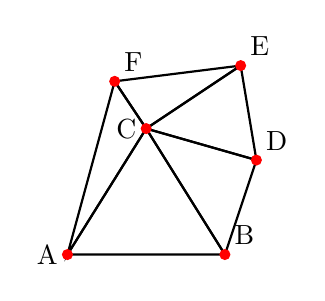
\begin{tikzpicture}
    % Punkte
    \coordinate (A) at (0,0);
    \coordinate (B) at (2,0);
    \coordinate (C) at (1,1.6);
    \coordinate (D) at (2.4,1.2);
    \coordinate (E) at (2.2,2.4);
    \coordinate (F) at (0.6,2.2);
    
    % Triangles (aus Delaunay-Triangulation)
    \draw[thick] (A) -- (B) -- (C) -- cycle;
    \draw[thick] (B) -- (C) -- (D) -- cycle;
    \draw[thick] (C) -- (D) -- (E) -- cycle;
    \draw[thick] (C) -- (E) -- (F) -- cycle;
    \draw[thick] (A) -- (C) -- (F) -- cycle;
    
    % Punkte markieren
    \foreach \p/\name in {A/A, B/B, C/C, D/D, E/E, F/F} 
    {
        \fill[red] (\p) circle (2pt);
    }    
    
    \node[left] at (A) {A};
    \node[above right] at (B) {B};
    \node[left] at (C) {C};
    \node[above right] at (D) {D};
    \node[above right] at (E) {E};
    \node[above right] at (F) {F};
\end{tikzpicture}

    \caption{Two-dimensional Delaunay triangulation used to illustrate shared
    interior edges.}
    \label{fig:2D_Delaunay_Triangulation}
\end{figure}

Let a set of points in $\mathbb{R}^2$ be connected via a Delaunay triangulation, as illustrated in \cref{fig:2D_Delaunay_Triangulation}. The triangulation satisfies the classical Delaunay criterion, whereby the circumcircle of each triangle contains no other point from the point set. While this property ensures geometric optimality in two dimensions, complications arise when this triangulation is used as the basis for iso-contouring in a lifted space $\mathbb{R}^{N+1}$, where each vertex is associated with a scalar value (e.g., height, potential, or another physical quantity).
The core issue stems from the fact that each interior $(N-1)$-face (e.g., edge in 2D, triangle in 3D) in a Delaunay triangulation is shared by exactly $N$ adjacent $N$-simplices in $\mathbb{R}^N$. For example, in the two-dimensional case ($N = 2$), each interior edge is shared by two adjacent triangles. When iso-contouring is performed in $\mathbb{R}^3$, i.e., with scalar lifting, the intersection of a level set (e.g., $f(\mathbf{x}) = 0$) with the mesh is computed by locating points along the edges of each triangle (or more generally, along the edges of each $N$-simplex) where the scalar field intersects the specified iso-value. This is typically done via linear root-finding: given two vertices $\mathbf{x}_i$ and $\mathbf{x}_j$ of an edge with associated scalar values $f_i = f(\mathbf{x}_i)$ and $f_j = f(\mathbf{x}_j)$, the intersection point $\mathbf{x}_\lambda$ satisfying $f(\mathbf{x}_\lambda) = f_{\text{iso}}$ is found by solving
%
\begin{equation}
    \lambda = \frac{f_{\text{iso}} - f_i}{f_j - f_i}, \quad \mathbf{x}_\lambda = (1 - \lambda)\mathbf{x}_i + \lambda \mathbf{x}_j.
\end{equation}
%
This process is repeated for each edge of the mesh that spans the iso-value, resulting in a piecewise linear approximation of the isosurface.

However, this leads to a structural redundancy: each interior edge contributes intersection points multiple times---specifically, once per adjacent simplex. In contrast, boundary edges appear only once in the triangulation and hence contribute only a single intersection, if any.

This redundancy leads to two principal problems:
\begin{enumerate}
    \item \textbf{Computational inefficiency:} Interior edges are processed $N+1$ times, resulting in redundant calculations. This inflates the number of computed contour segments, increases memory requirements, and slows down the iso-contouring algorithm.
    
    \item \textbf{Statistical bias:} If a statistical measure (e.g., the arithmetic mean) is computed over the set of intersection points, the interior edges are overrepresented by a factor of $N+1$, while boundary edges are represented only once. Consequently, the result is a biased estimate. For example, the mean of all intersection points is shifted toward the interior, which may lead to incorrect physical interpretations such as distorted center-of-mass calculations or erroneous gradient approximations.
\end{enumerate}

Thus, although Delaunay triangulations are optimal with respect to angle quality and avoidance of narrow triangles, their direct use in higher-dimensional scalar field interpolation introduces a fundamental asymmetry. To ensure accuracy and efficiency in iso-contouring or zero-level set extraction, it is imperative to apply either:

\begin{itemize}
    \item an \emph{edge-level de-duplication} strategy, wherein each edge is processed exactly once, or
    \item a \emph{post-processing normalization}, such as weighting the contribution of each intersection point inversely with its multiplicity in the triangulation.
\end{itemize}

Failure to address this issue may result in significant deviations from the true geometry or statistics of the underlying physical field, particularly when global operations (e.g., integration, averaging) are applied.
